%\documentclass[]{algotel}
%\usepackage[utf8]{inputenc}

%\usepackage{xspace}
%\usepackage{graphicx,graphics} 
%\usepackage{mathtools, bm}
%\usepackage{caption}
%\usepackage{amssymb, bm}
%\usepackage{complexity}
%\usepackage{amsthm}
%%\usepackage{authblk}
%\usepackage{color}
%\usepackage{amsmath}
%\usepackage[colorlinks=true,breaklinks=true,linkcolor=blue]{hyperref}
%\captionsetup{justification=centering,margin=0.5cm}
\documentclass[]{llncs}
%
\usepackage[utf8]{inputenc}
\usepackage[english]{babel}
\usepackage{caption}

\usepackage{graphicx}

\newcommand\pall{\textsc{pall}\xspace}
\newcommand{\todo}[1]{{\color{red} TODO: {#1}}}	
\newtheorem{prop}{Proposition}
\renewcommand{\thefootnote}{\*}

\graphicspath{{img/}}
\title{Contention management for Cloud RAN over an optical ring}
\author{Dominique Barth \inst{1}
  \and Ma\"el Guiraud \inst{1}
   \and Yann Strozecki \inst{1}
  }

\institute{David Laboratory, UVSQ}



\begin{document}

\maketitle


\begin{abstract}
The N-GREEN project has for goal to design a low cost optical ring technology with good performances (throughput, latency$\dots$) without using expensive end to end connections. We study the compatibility of such a technology with the development of the Cloud RAN, a latency critical application which is a major aspect of 5G deployment. We show that deterministically managing Cloud RAN traffic minimizes its latency while also improving the latency of the other traffics. 
\keywords{Optical ring \and Latency \and C-RAN \and SDN}
\end{abstract}


\section{Introduction}

\footnote{This work was developed around the ANR N-GREEN project. The authors thank the Nokia Bell Labs team for their collaboration.}Network providers have to design inexpensive networks supporting an increasing amount of data and online applications. Much of these applications have QoS criteria, like a minimal throughput or a maximal latency. The N-GREEN project aims to design a high performing optical ring while ensuring a minimal cost for providers. The current solutions with good QoS~\cite{pizzinat2015things,tayq2017real}, establish end to end direct connections (E2DE) between the nodes, which is extremely expensive. The N-GREEN optical ring is designed to ensure good performance: the hardware it requires scales linearly with the number of nodes while E2DE scales quadratically making it impractical for more than a few nodes.

In this article, we study a Cloud RAN (C-RAN) application based on the N-GREEN optical ring described in~\cite{ngreenarchitecture,uscumlicscalable}. C-RAN is one of the major area of development for 5G; it consists in centralizing or partially centralizing the computation units or {\bf BaseBand Units} (BBU) of the {\bf Remote Radio Heads} (RRH) in one datacenter. The latency of the messages between the BBU and the RRH is critical since some services need end-to-end latency as low as $1$ms~\cite{3gpp5g,boccardi2014five}. In this article we propose an SDN approach to deterministically manage the periodic C-RAN traffic by choosing emission timing and reserving containers on the ring. In a previous work~\cite{dominique2018deterministic}, the authors have studied a similar problem for a star shaped network. In contrast with our previous work, finding emission timings so that different periodic sources do not use the same resource is easy in the context of the N-GREEN optical ring. However, we add several new difficulties: the messages from RRHs are scattered, there are other traffics whose latency must be preserved and the need to make reservation of containers on the ring requires additional bandwidth.

In Sec.~\ref{sec:model}, we model the optical ring and the traffic flow. In Sec.~\ref{sec:oportmethods}, we experimentally evaluate the latency when using stochastic multiplexing to manage packet insertions on the ring, with or without priority for C-RAN packets. In Sec.~\ref{sec:deterministicalgorithms}, we propose a deterministic way to manage C-RAN packets without buffers, which guarantee to have zero latency from buffering. We propose several refinements of this deterministic sending scheme to spread the load over time, which improves the latency of best effort packets.

\section{Model of C-RAN traffic over an optical ring}
\label{sec:model}
    
  \paragraph{N-GREEN Optical ring}
   
  The unidirectional optical ring is represented by an oriented cycle. The vertices of the cycle represent the nodes of the ring, where the traffic arrives. The edges $(u,v)$ of the cycle have an integer weight $\omega(u,v)$ which represents the time to transmit a unit of information from $u$ to $v$. By extension, if $u$ and $v$ are not adjacent, we denote by $\omega(u,v)$ the size of the directed path from $u$ to $v$.  The \textbf{ring size} is the length of the cycle, that is $\omega(u,u)$ and we denote it by $RS$. A {\bf container}, of capacity $C$  expressed in bytes, is a basic unit of data in the optical ring. 
  
  A unit of time corresponds to the time needed to fill a container with data:
  The node $u$ can fill a container with a data packet of size less than $C$ bytes at time $t$ if the container 
  at position $u$ at time $t$ is \emph{free}. A container goes from $u$ to $v$ in $\omega(u,v)$ units of time. The ring follows a {\bf broadcast and select scheme with emission release policy}: When a container is filled by some node $u$, it is freed when it comes back at $u$ after a whole round trip.
  
  \begin{figure}[h!]
       \begin{minipage}[b]{0.5\linewidth}
        \begin{center}
      \includegraphics[scale=0.7]{containers}
   
      \end{center} 
  \end{minipage}
    \begin{minipage}[b]{0.5\linewidth}
        \begin{center}
      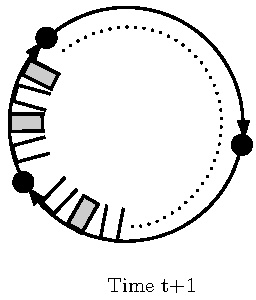
\includegraphics[scale=0.7]{containers2}
      

      \end{center} 
  \end{minipage}
   
     \caption{Behavior of the containers on the ring.}\label{fig:containers}

  \end{figure}
  
     \paragraph{C-RAN traffic}
   
   The RRHs are the source of the {\bf deterministic and periodic} C-RAN traffic.
   There are $n$ RRHs attached to the ring and several RRHs can be attached to the same vertex. An RRH is linked to a node of the ring through an electronic interface of bit rate $R$ Bps.
   The ring has a larger rate of $F\times R$ Bps. The integer $F$ is called the {\bf acceleration factor} between the electronic and the optical domains. A node aggregates the data received on the electronic interface during $F$ units of time to create a packet of data of size $C$ and then fills a container of the ring with this data. 
  In each period $P$, an RRH emits data during a time called \textbf{emission time} or $ET$. Hence the RRH emits $ET / F$ packets, i.e. a container of size $C$ each $F$ units of time during the emission time, see Fig.~\ref{fig:interface}.
   %Each period $P$, an RRH emits $ET / F$ packets, i.e. a packet of size $C$ each $F$ units of time during a time $ET$ (emission time),
   
   The data of the RRH $i$ arrives at some node $u$ at a time $m_i$ called {\bf offset}. The offsets can be determined 
   by the designer of the system and can be different for each RRH but must remain the same over all periods. We assume that all BBUs are contained in the same data-center attached to the node $v$. The data from $u$ is routed to its BBU at node $v$ through the ring and arrives at time $m_i + \omega(u,v)$ if it has been inserted in the ring upon arrival. Then after some computation time (which w.l.o.g. is supposed to be zero), an answer is sent back from the BBU to the RRH. The same quantity of data is emitted by each BBU or RRH during any period.
   In this study the {\bf latency} of a message is defined as the time it waits in a node before being sent on the ring.
   The aim of our study is to minimize the latency of the C-RAN traffic, both of the RRHs and the BBUs. 
   In Sec.~\ref{sec:deterministicalgorithms} we propose a deterministic mechanism with zero latency which preserves the latency of other data using the optical ring. We shortly describe the nature of this additional traffic in the next subsection.
   
    
\begin{figure}[h!]
\begin{center}   

      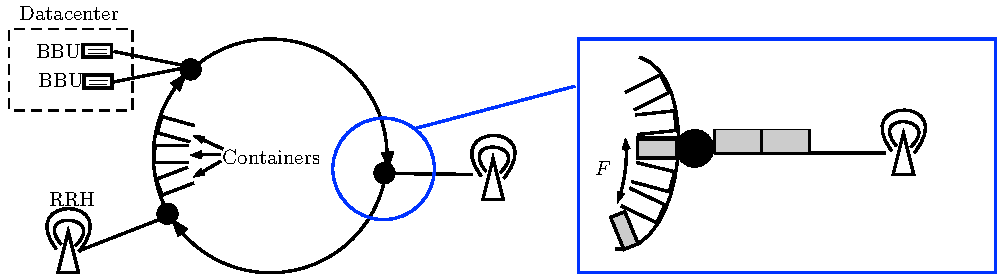
\includegraphics[scale=0.7]{interface.pdf}
     \caption{Access node of the N-GREEN optical ring.}\label{fig:interface}
     
\end{center}
  \end{figure}


\paragraph{Best effort traffic}

The optical ring supports other traffics, corresponding to the internet flow. We call this traffic \textbf{Best Effort} (BE). We want it to have the best possible distribution of latency, but since BE traffic is less critical than C-RAN traffic, we impose no hard constraint on its latency. At each node of the ring, a contention buffer is filled by a batch arrival process of BE data. Then according to some parameters, fill rate and maximum waiting time, data on the contention buffer are aggregated in a packet of size at most $C$. The node fills a container on the ring with this packet as soon as possible. Hence, the arrival of BE messages is modeled by a temporal law that gives the distribution of times between two arrivals of a packet of BE messages in a node. The computation of this distribution for the parameters of the contention buffer used in the N-GREEN optical ring is described in ~\cite{youssef2018}.

   \section{Evaluation of the latency on the N-GREEN optical ring}
   \label{sec:oportmethods}
   
   
  We first study the latency of the C-RAN and BE traffics when the ring follows an opportunistic insertion policy: When a node wants to fill some container, it does it as soon as it can. 
  If there are several data packets in a node or if a node cannot fill a container, because it is not free, 
  the remaining packets are stored in an insertion buffer. Two different methods to manage this insertion buffer are experimentally compared. The FIFO rule is compared to a method that uses two insertion buffers: one for the BE packets, and another for the C-RAN packets. The C-RAN insertion buffer first has the priority and is used to fill containers on the ring while it is non empty before considering the BE insertion buffer.  Fig.~\ref{fig:resultopport} gives the cumulative distribution of both C-RAN and BE traffics latencies for the FIFO rule and the "C-RAN first" rule. In this experiment, the offsets of the RRH are not fixed but randomly distributed in the period. The experimental parameters are given by Fig.~\ref{fig:params} and chosen following~\cite{ngreenarchitecture}. The results are computed over $100$ experiments (with different random offsets) where the optical ring is simulated during $10,000,000$ units of time. The source code in C of the experiments can be found on one of the authors webpage~\cite{webpage}.
  
   \vspace{0.5cm}
  \hspace{-0.75cm}
    \begin{minipage}[b]{0.50\linewidth}


        \begin{center}
      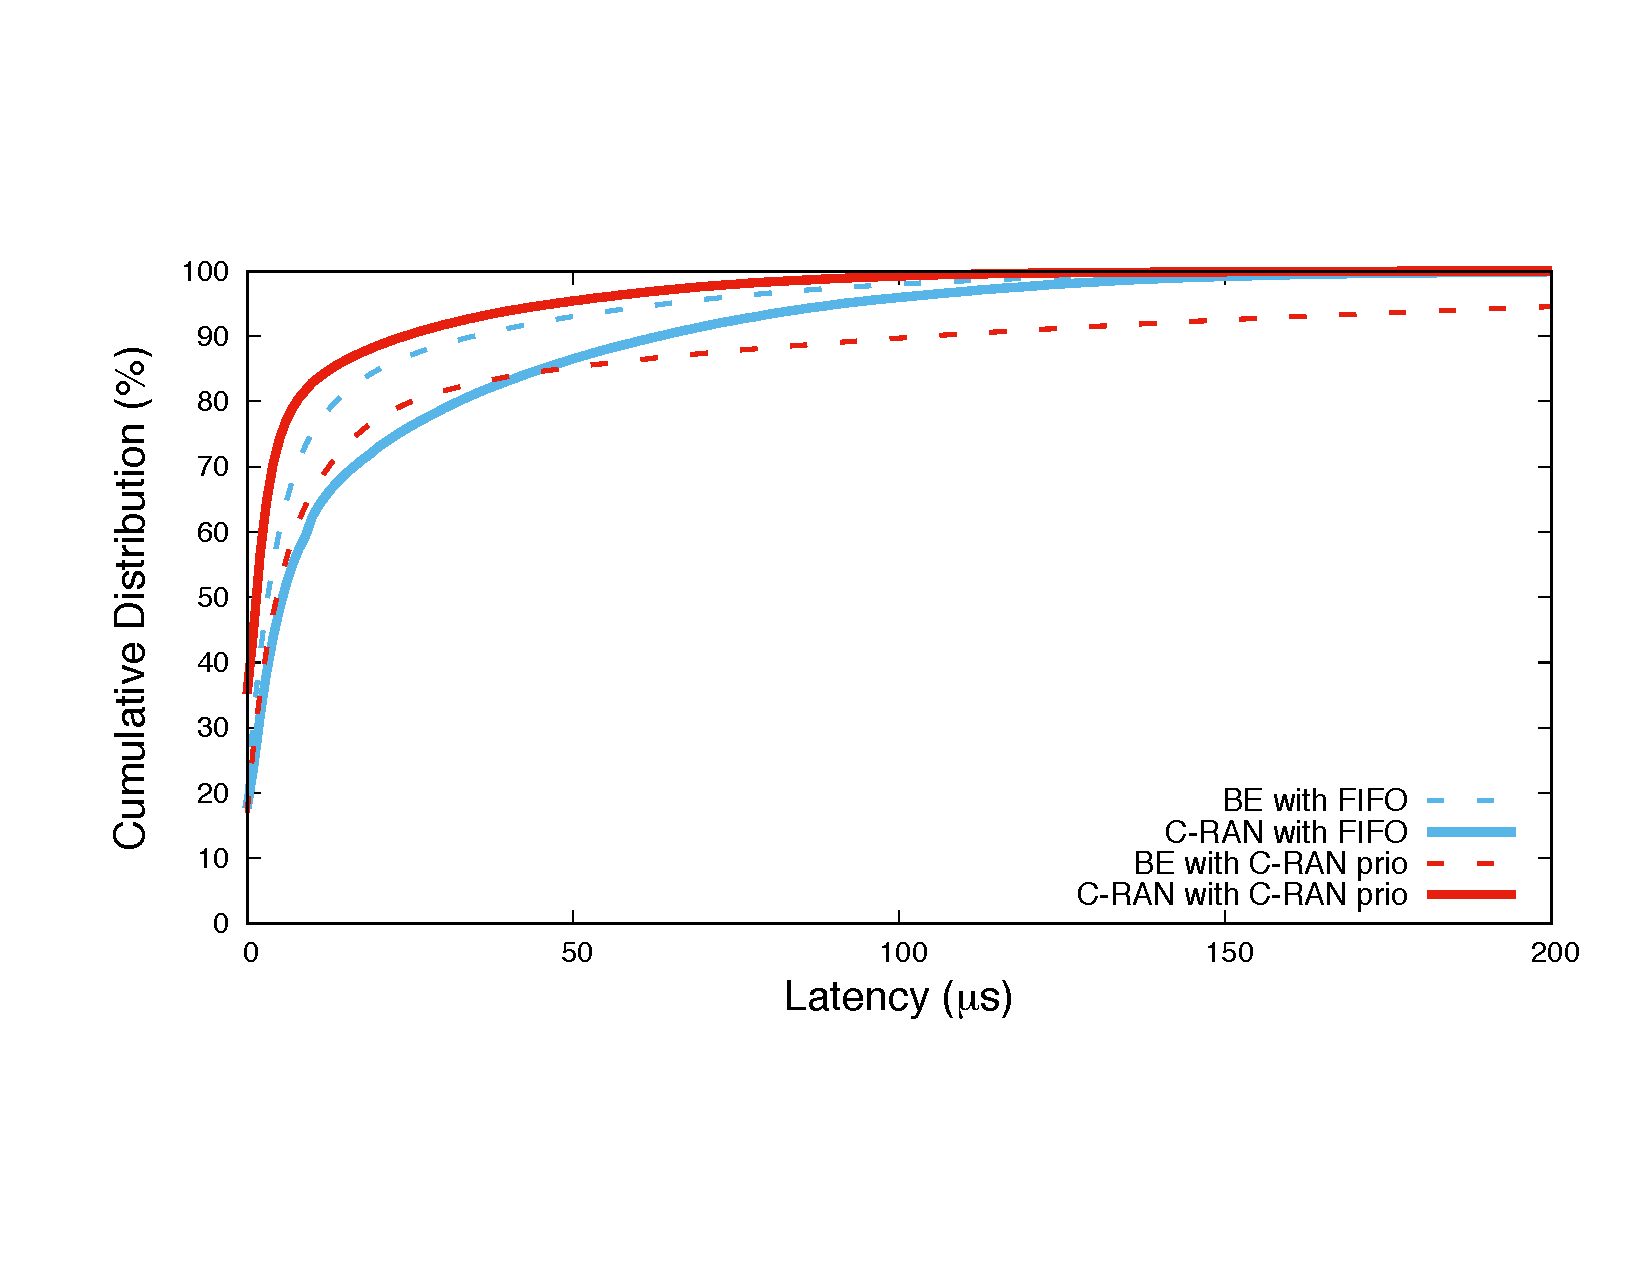
\includegraphics[scale=0.3]{opport.pdf}

     \captionof{figure}{Distribution of latencies for FIFO and C-RAN first}    \label{fig:resultopport}
      \end{center} 
  \end{minipage}
\hfill
  \begin{minipage}[b]{0.40\linewidth}
 
  \scalebox{0.65}
  {
 
  \centering
  \begin{tabular}{|c|c|}
  \hline
  Bit rate of an electronic interface $R$ & $10$ Gbps \tabularnewline
  \hline
  Optical ring bit rate $F\times R$ & $100$ Gbps \tabularnewline
  \hline
    Acceleration factor $F$ & $10$  \tabularnewline
  \hline
  Container size  $C$ & $100$ kb  \tabularnewline
  \hline
  Unit of time $C/(F\times R)$ & $1~\mu$s \tabularnewline
  \hline
  Length of the ring $RS$ & $100$ \tabularnewline
  \hline
  Emission time $ET$ & $500$ \tabularnewline
  \hline
   Period $P$ & $1,000$ \tabularnewline
  \hline
  Number of RRH & $5$  \tabularnewline
  \hline
  Number of nodes $n$ & $5$  \tabularnewline
  \hline
   Load induced by C-RAN traffic & $50\%$  \tabularnewline
  \hline
    Load induced by BE traffic & $40\%$  \tabularnewline
  \hline
  \end{tabular}
  }

  \captionof{figure}{Experimental parameters of the N-GREEN architecture}\label{fig:params}

  \end{minipage} 
  
Unsurprisingly, the latency of the C-RAN traffic is better when we prioritize the C-RAN messages, while the BE traffic is penalized. Nevertheless, there is still $10\%$ of the C-RAN traffic with a latency higher than $50 \mu$s, a problem we address in the next section.


\section{Deterministic approach for zero latency} \label{sec:deterministicalgorithms}

Finding good offsets for the C-RAN traffic is a hard problem even for simple topologies and without BE traffic, see~\cite{dominique2018deterministic}. In this section, we give a simple solution to this problem in the N-GREEN optical ring, and we adapt it to minimize the latency of the BE traffic.

Let $u$ be the node to which is attached the RRH $i$, to ensure zero latency for the C-RAN traffic, then the container which arrives at $u$ at time $m_i$ must be free so that the data from the RRH can be sent immediately on the optical ring. 

To avoid latency between the arrival of the data from the RRH and its insertion on the optical ring, 
we allow nodes to \textbf{reserve} a container one round before using it. A container which is reserved cannot be filled by any node except the one which has reserved it (but it may contain data when it is reserved). 
Let $u$ be the node to which is attached the RRH $i$, if $u$ reserves the container $u$ at time $m_i - RS$, then it is guaranteed that $u$ can fill a free container at time $m_i$ with the data of the RRH $i$.
In the method we now describe, the C-RAN packets never wait in the node: The message sent by the RRH $i$ arrives at its BBU at node $v$ at time $m_i + \omega(u,v)$ and the answer is sent from the BBU at time $m_i + \omega(u,v) +1$.

Recall that an RRH fills a container every $F$ units of time, during a time $ET$. 
Thus if we divide the period $P$ into \textbf{slots} of $F$ consecutive units of time, an RRH needs to use at most one container by slot. If an RRH emits at time $m_i$, then we say it is at \textbf{position} $m_i + \omega(u,v)\pmod F$. 
The position of an RRH corresponds to the position in a slot of the container it has emitted, when it arrives at $u$. 
If an RRH is at position $p$, then by construction, the corresponding $BBU$ is at position $p+1\pmod F$. Since we do not allow waiting times for C-RAN traffic, each RRH uses a container at the same position during all the period. 

The problem we solve now is to find an \textbf{assignment} of values of the $m_i$'s which is \textbf{valid}: two RRHs never reserve or use the same container in a period. Moreover we want to preserve the latency of the BE traffic. It means that the time a node waits for a free container at any point of the period must be minimized. 
Remark that two RRHs which are not at the same position never use the same containers. Moreover, if we fix the offsets of the RRHs to even positions so that they do not reserve the same containers, then it will fix the offsets of the BBUs to odd positions which do not reserve the same containers. Hence we need to deal with the RRHs only.


\begin{prop}
\label{prop:assign}
There is an assignment of the offsets $m_1, \dots, m_k$ on the same position if  $k\times ET + RS \leq P$.
\end{prop}
\begin{proof}
 W.l.o.g we fix $m_1$ so that it is at position $0$ and all the other offsets will then be chosen at position $0$. 
 Let $u_1,\dots,u_k$ be the nodes attached to the RRHs $1,\dots,k$. We assume that $u_1,\dots,u_k$ are in the order of the ring. The last message emitted by the RRH $1$ arrives at $u_2$ at time $ET - 1 + \omega(u_1,u_2)$. Therefore we can fix $m_2 =  ET  + \omega(u_1,u_2)$. In general we can set $m_i = (i-1) \times ET + \omega(u_1,u_i)$ and all RRHs will use different containers at position $0$ during a period. Since $k \times ET + \omega(u_1,u_1) \leq P$ by hypothesis,
 the containers filled by the $k$th RRH are freed before $P$. Hence when the RRH $1$ must emit something in the second period, there is a free container.\qed
\end{proof}

From this proposition, it is easy to derive the maximal number of antennas which can be supported by an optical ring,
when using reservation and the same position for an RRH for the whole period.

\begin{corollary}
The maximal number of antennas such that there is an assignment is $ \lfloor\frac{P- RS}{ET}\rfloor \times \frac{F}{2}$.
\end{corollary}
\begin{proof}
Following Prop.~\ref{prop:assign}, the number of antennas on a position is $k = \lfloor\frac{P- RS}{ET}\rfloor $.
Since we need two positions for $k$ antennas, in order to carry the traffic coming from the RRHs and the BBUs, and we got $F$ positions in the slot, the number of antennas supported by the ring is thus equal to $k \times \frac{F}{2}$.\qed
\end{proof}

We now present an algorithm to determine an assignment of the $m_i$, using the method of Prop.\ref{prop:assign} to set the offset at the same positions. We propose three variations to optimize the latency of the BE traffic, by spacing as well as possible the free containers in a period. 


\paragraph{Packing}

For each position which is used by some RRH, and during each period, $RS$ containers are reserved before starting to emit some C-RAN traffic, while they are free. Hence, it decreases the maximal load the system can handle.
Therefore to not waste bandwidth, it is relevant to put as many RRHs as possible on the same position as in Fig.~\ref{fig:repart0}. Indeed, for any position which is not used at all, $RS$ containers need not to be reserved. This strategy is also good for the latency of the BE traffic. If a position is unused, then there is always a container free of C-RAN traffic each $F$ unit of times. 

\begin{figure}[h!]
\begin{center}   

      \includegraphics[scale=0.55]{repart0}
     \caption{Packing.}\label{fig:packing}
     
\end{center}
  \end{figure}

\paragraph{Balancing inside the slot}

The free positions can be distributed uniformly over a slot, to minimize the time to wait before a node 
has access to a free container, as shown in Fig.~\ref{fig:repart1}. It is a small optimization, since 
it decreases the latency of at most $F/2$.

\begin{figure}[h!]
\begin{center}   

      \includegraphics[scale=0.55]{repart1}
     \caption{Balancing inside the slot.}\label{fig:packing}
     
\end{center}
  \end{figure}
\paragraph{Balancing inside the period}

It is possible that there are no unused position as it happens with the parameters of the N-GREEN ring given in Fig.~\ref{fig:params}: $ET = \frac{P}{2}$, $F = 10$ and $n = 5$. Any assignment has exactly one  BBU or RRH at each position. If all the RRHs start to emit in the first slot, then during $ET$ there will be no free containers anywhere on the ring, inducing a huge latency for the BE traffic. 
To mitigate this problem, in a period, the time with free containers in each position must be uniformly distributed over the period as shown in Fig.~\ref{fig:repart2}.
\begin{figure}[h!]
\begin{center}   

      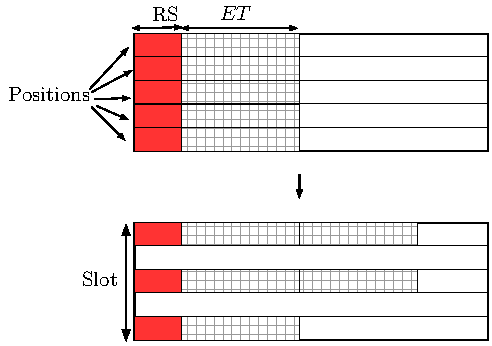
\includegraphics[scale=0.55]{repart2}
     \caption{Balancing inside the period.}\label{fig:packing}
     
\end{center}
  \end{figure}  
  \paragraph{Experimental evaluation}

  In order to understand the contribution of the three ideas presented in the previous subsection,
   we present the cumulative distribution of the latency of the BE traffic latency in Fig.~\ref{fig:algocmp}. Since the previous N-GREEN parameters were too restrictive to put several RRHs on the same position, the parameter $ET$ has been changed to $400$.

The performance when we do no packing is really bad, even worst than the methods using an insertion buffer. It is explained by the parameters of the N-GREEN ring: all positions are used and thus, there are no free containers available to BE traffic during $ET+RS$ units of time. When packing the RRHs on a minimal number of positions, the latency decreases dramatically and becomes much better than in the previous methods. The optimizations of spacing inside the slot brings almost no benefit as expected. The spacing over a period improves the latency marginally. In settings with an higher load, spacing inside a period would have a much larger effect.

In Fig.~\ref{fig:optimres}, we compare the cumulative distribution of the latency of the BE traffic using the FIFO rule or the reservation algorithm proposed here. To keep the load at $90\%$ as in the experiment of Fig.~\ref{fig:resultopport}, we set $ET = 200$ and $n = 12$. This is not out of context since the exact split of the C-RAN (the degree of centralization of the computation units in the cloud) is not fully determined yet~\cite{mobile2011c}. With these parameters, the loss of bandwidth due to reservation is at most $6\%$
 

  \begin{minipage}[b]{0.45\linewidth}
\centering
      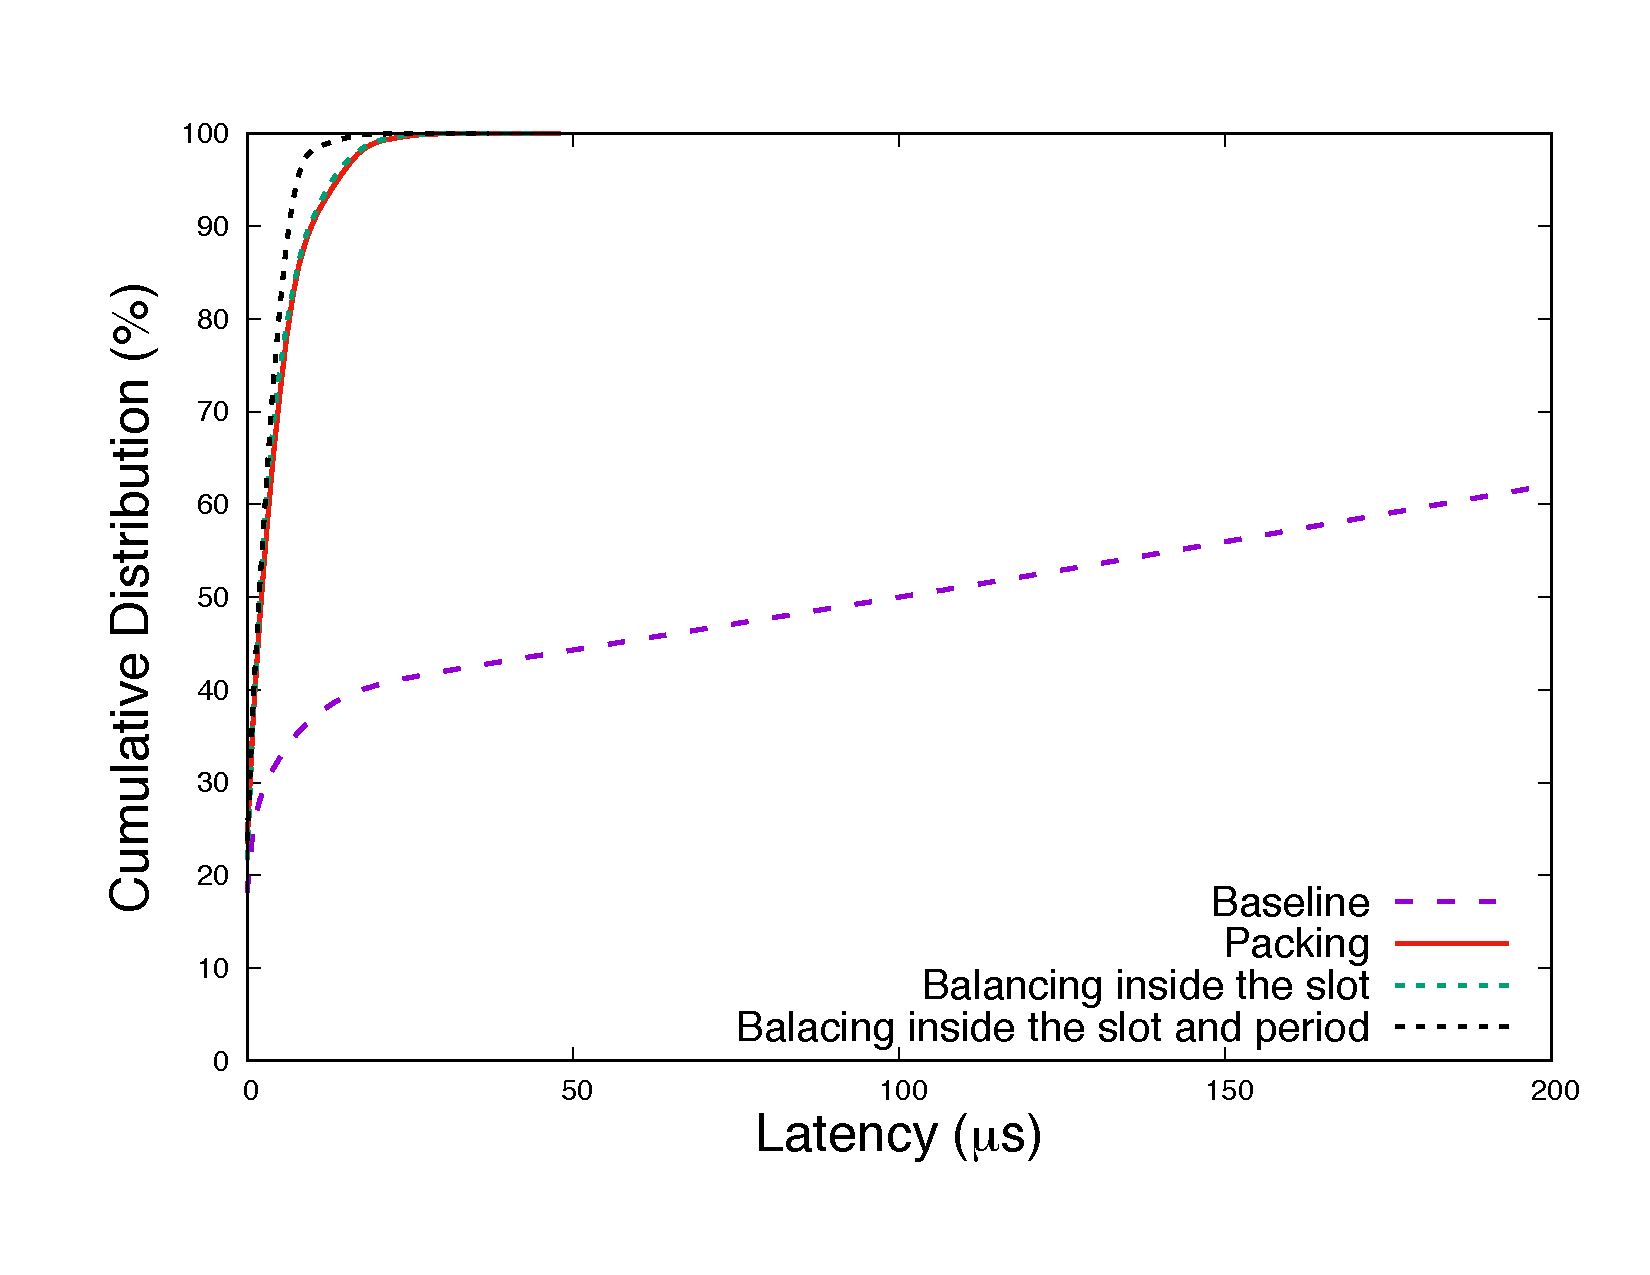
\includegraphics[scale=0.25]{repart1res}
     \captionof{figure}{Impact of the repartition on the latency.}   \label{fig:algocmp}
  \end{minipage} 
  \hfill
  \begin{minipage}[b]{0.45\linewidth}
\centering
      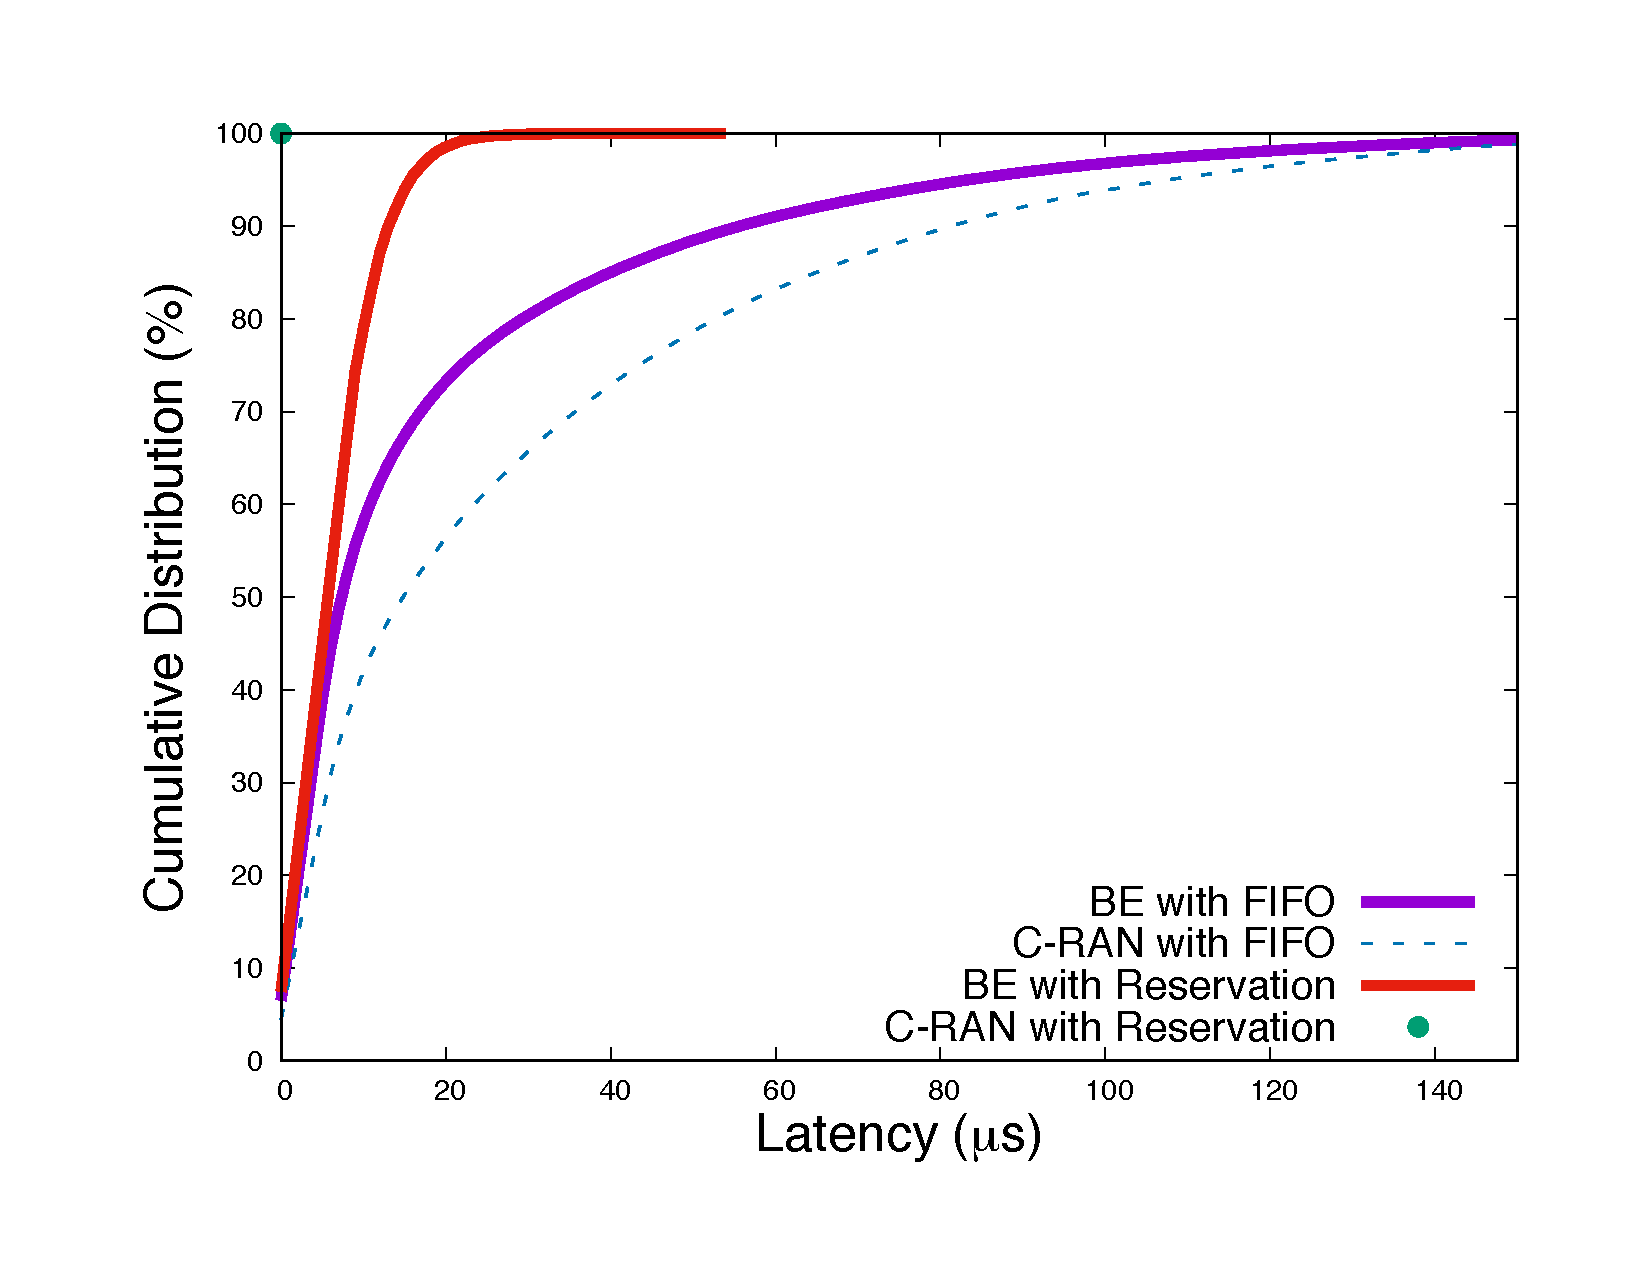
\includegraphics[scale=0.25]{optim.pdf}
     \captionof{figure}{Impact of the deterministic method on the traffics.}   \label{fig:optimres}
  \end{minipage} 


  The performance of the reservation algorithm is excellent, since the C-RAN traffic has {\bf zero latency} and the BE traffic has a \textbf{better latency} with reservation than with the FIFO rule. It is due to the balancing of the load of the C-RAN traffic over the period, that guarantee a more regular bandwidth for the BE traffic.
  

  
  \bibliographystyle{ieeetr}
\bibliography{src}

\end{document}
